% ==========================================
% Section 3: Missing Values (Slides 8-12)
% ==========================================

% Slide 8: Missing Values Reasons
\begin{frame}{مقادیر گمشده / ازدست‌رفته}
\begin{columns}[c]
  \begin{column}{0.58\textwidth}
    \begin{itemize}
      \item \textbf{دلایل احتمالی فقدان مقادیر:}
      \begin{itemize}
        \item قطع موقت ارتباط یا خرابی حسگر
        \item از بین رفتن بسته‌های داده در حین انتقال شبکه
        \item عدم گردآوری یا ثبت اطلاعات در منبع اولیه
        \item عدم پاسخ مشتریان به پرسش‌های اختیاری در فرم‌ها
        \item عدم وجود ویژگی در برهه زمانی ثبت رکورد
      \end{itemize}
    \end{itemize}
  \end{column}
  \begin{column}{0.40\textwidth}
    \centering
    
\includegraphics[width=\textwidth]{images/page_08_img_1.png}
  \end{column}
\end{columns}
\end{frame}

% Slide 9: Missing Values Treatments
\begin{frame}{مقادیر گمشده: راهکارهای حذف و جایگزینی}
\begin{itemize}
  \item \textbf{روش‌های مواجهه با مقادیر گمشده (\lr{Treatments}):}
  \begin{itemize}
    \item \textbf{حذف رکوردهای دارای نقص در داده‌های آموزش (\lr{Deletion}):} نادیده گرفتن سطرها
    \item \textbf{جایگزینی مقادیر (\lr{Imputation}):}
    \begin{itemize}
      \item مقدار پیش‌فرض یا برچسب مشخص (مانند \lr{0} یا \lr{"missing"})
      \item میانگین یا میانه برای متغیرهای عددی (\lr{Mean / Median})
      \item بیشترین فراوانی برای متغیرهای اسمی (\lr{Mode})
    \end{itemize}
    \vspace{0.05cm}
    \codebox{SimpleImputer(missing\_values=np.nan, strategy='mean')}
    \vspace{0.05cm}
    \item \textbf{تلاش برای پیش‌بینی هوشمند مقادیر گمشده:}
    \begin{itemize}
      \item در نظر گرفتن تخمین مقادیر مفقود به عنوان یک مسئله یادگیری ماشین
      \item \textbf{هدف (\lr{Target}):} متغیری که مقدار گمشده دارد
      \item \textbf{داده‌های آموزش:} رکوردهایی که متغیر در آن‌ها وجود دارد
      \item \textbf{داده‌های آزمون:} رکوردهایی که متغیر در آن‌ها مفقود است
    \end{itemize}
    \vspace{0.05cm}
    \codebox{KNNImputer(n\_neighbors=2, weights="uniform")}
  \end{itemize}
\end{itemize}
\end{frame}


% Slide 10: Missing Values Caveats
\begin{frame}{مقادیر گمشده: تصادفی در برابر غیرتصادفی}
\begin{itemize}
  \item \textbf{نکته کلیدی: مقادیر به دلایل گوناگون گم می‌شوند:}
  \begin{itemize}
    \item بسیار مهم: آیا گم‌شدگی تصادفی است یا غیرتصادفی؟ (\lr{Random vs. Not at Random})
  \end{itemize}
  \vspace{0.2cm}
  \item \textbf{نمونه‌هایی از گم‌شدگی غیرتصادفی (\lr{Not at Random}):}
  \begin{itemize}
    \item سوالات اختیاری حساس در پرسشنامه‌ها (مثلاً «میزان درآمد سالیانه» یا «مصرف دخانیات»)
    \item مقادیری که فقط تحت شرایط خاص تعریف می‌شوند (مثلاً «معدل مدرک ارشد»)
    \item متغیرهایی که تنها به بخش خاصی از جامعه مربوط می‌شوند (مثلاً «وضعیت بارداری»)
    \item حسگرهایی که در شرایط حدی (دمای بسیار بالا یا فشار شدید) دچار قطعی می‌شوند
  \end{itemize}
  \vspace{0.2cm}
  \item \textbf{در این سناریوها، پر کردن داده با میانگین منجر به از بین رفتن اطلاعات حیاتی می‌شود!}
  \begin{itemize}
    \item به بیان دیگر: \textbf{«گمشده بودن» خود یک سیگنال اطلاعاتی معنادار است!}
  \end{itemize}
\end{itemize}
\end{frame}

% Slide 11: Medical Trial Example
\begin{frame}{مدیریت مقادیر گمشده: ملاحظات و ریسک‌ها}
\begin{itemize}
  \item یک کارآزمایی بالینی برای بررسی عوارض جانبی یک داروی خاص را در نظر بگیرید:
  \item در این آزمایش، ۵۰ نفر مقدار قند خون خود را می‌دانند و گزارش کرده‌اند؛
  \begin{itemize}
    \item از میان آن‌ها، $4/5$ نفر قند خون بالا دارند.
  \end{itemize}
\end{itemize}
\vspace{0.1cm}
\centering
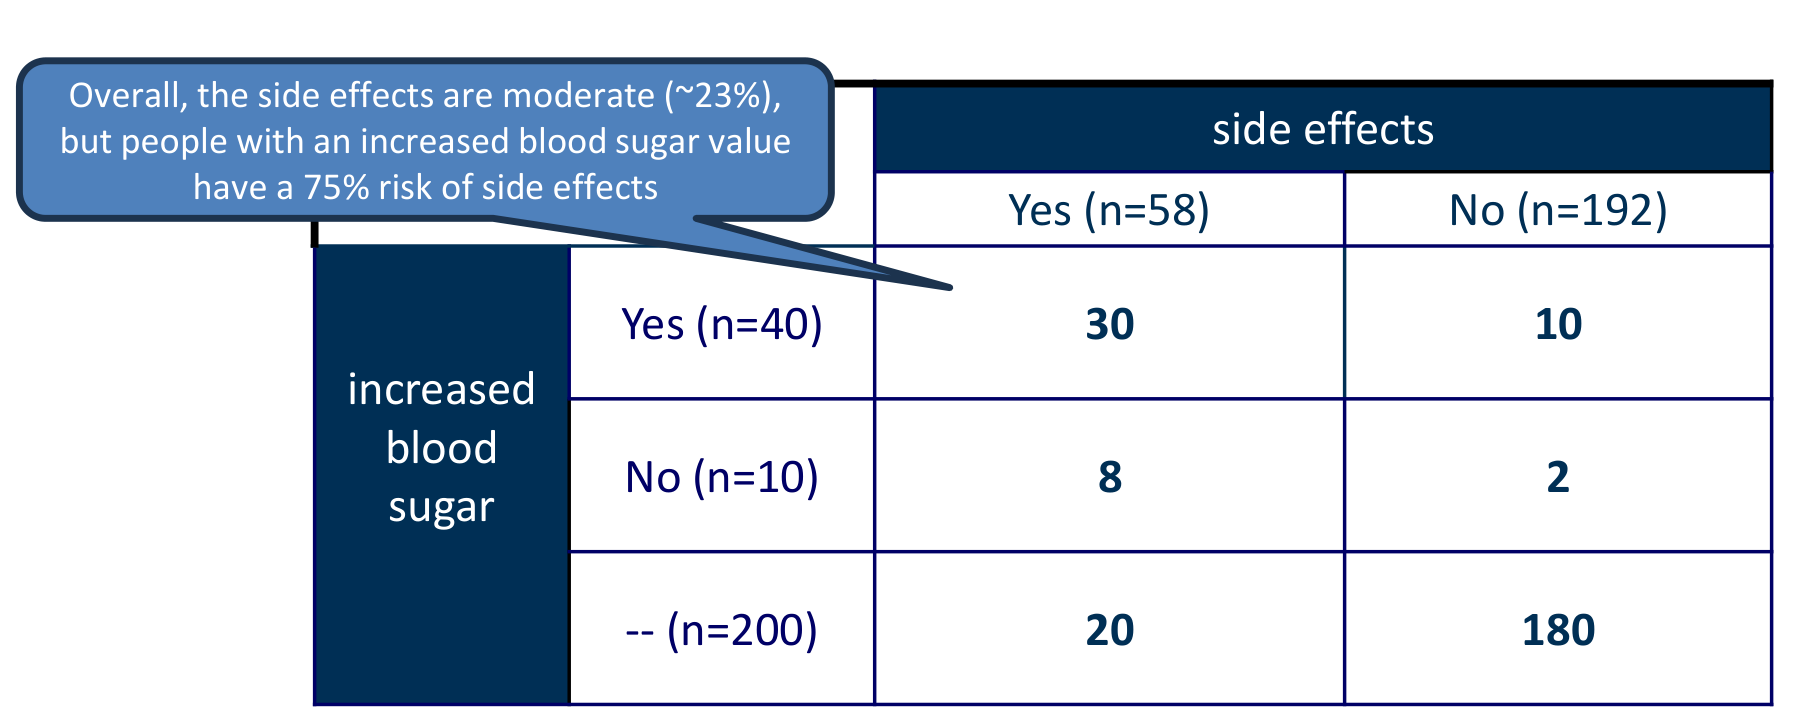
\includegraphics[width=0.72\textwidth]{images/page_11_table.png}
\vspace{0.1cm}
\begin{itemize}
  \item به طور کلی عوارض جانبی معتدل است (\lr{\textasciitilde 23\%})، اما افراد با قند خون بالا ریسک \lr{75\%} برای ابتلا به عوارض دارند.
\end{itemize}
\end{frame}

% Slide 12: Medical Trial Imputation Impact
\begin{frame}{مدیریت مقادیر گمشده: ملاحظات و ریسک‌ها (ادامه)}
\begin{itemize}
  \item فرض کنید مقدار گمشده قند خون بالا را با مقدار اکثریت («بله») پر کنیم:
\end{itemize}
\vspace{0.1cm}
\centering
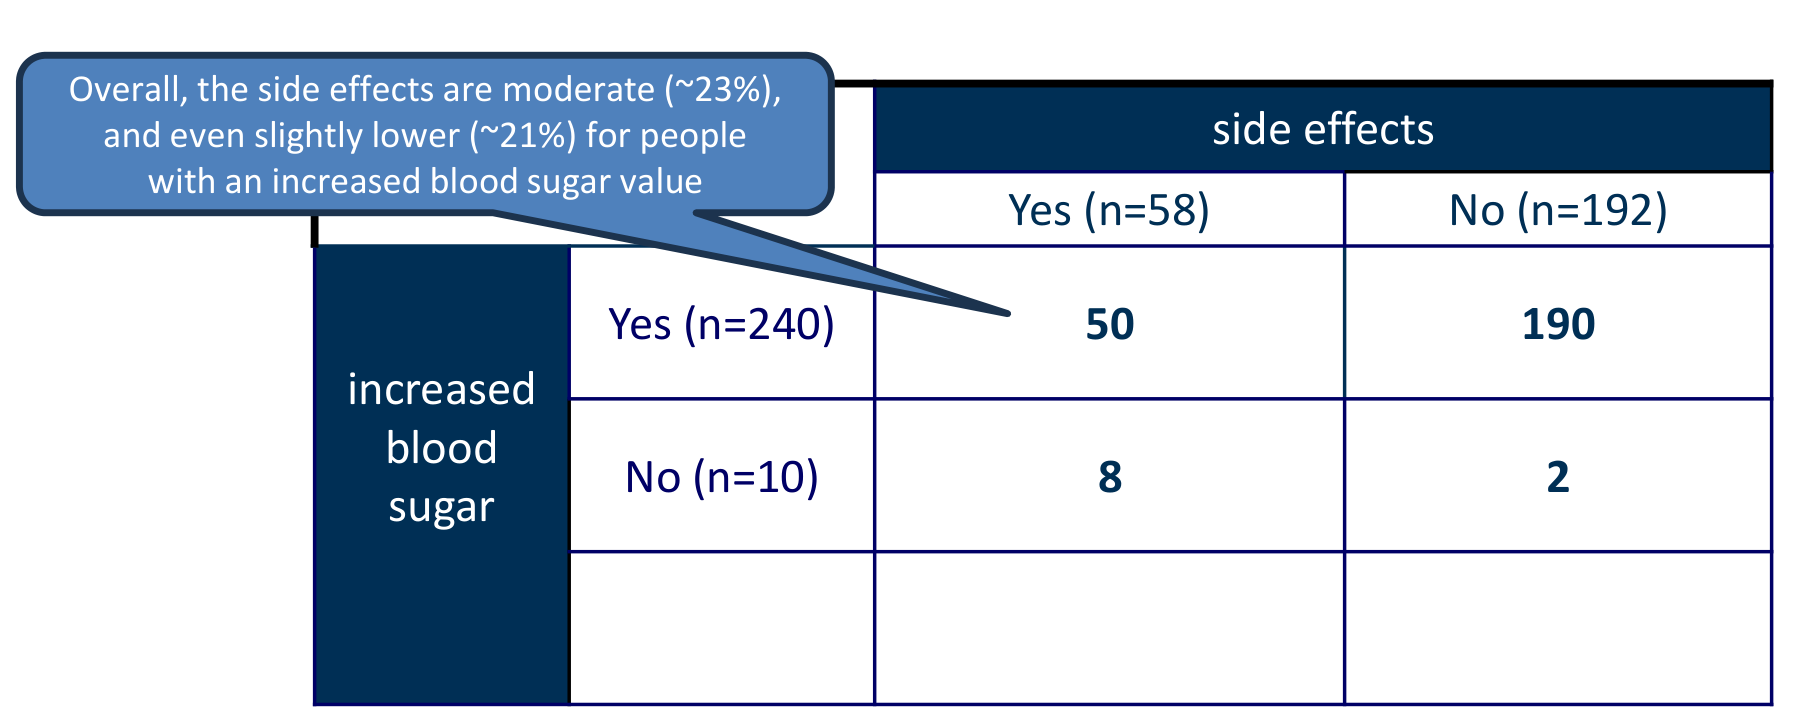
\includegraphics[width=0.72\textwidth]{images/page_12_table.png}
\vspace{0.1cm}
\begin{itemize}
  \item در کل عوارض جانبی معتدل باقی می‌ماند (\lr{\textasciitilde 23\%})، اما ریسک برای افراد با قند خون بالا از \lr{75\%} به \lr{\textasciitilde 21\%} کاهش می‌یابد (نتیجه کاملاً گمراه‌کننده)!
\end{itemize}
\end{frame}
